\documentclass[reprint, amsmath, amssymb, aps, pra, nofootinbib]{revtex4-2}

% --- Основные пакеты ---
\usepackage[T2A]{fontenc}
\usepackage[utf8]{inputenc}
\usepackage[russian,english]{babel}

\usepackage{graphicx}
\graphicspath{{figures/}}
\usepackage{bm}

% hyperref в REVTeX
\usepackage[unicode, colorlinks=true, linkcolor=blue, citecolor=blue, urlcolor=blue]{hyperref}

\begin{document}

\title{3.3.4 Эффект Холла в полупроводниках}

\author{Ефим Сычев}
\email{sychev.ea@phystech.edu}
\affiliation{Московский физико-технический университет, группа Б02-506}

\date{\today}

\begin{abstract}
Исследован эффект Холла в образце легированного германия в геометрии мостика Холла.
Проведена градуировка электромагнита и сняты зависимости поперечной разности потенциалов от индукции магнитного поля при различных токах через образец.
По знаку ЭДС Холла установлен дырочный тип проводимости ($p$-тип) и найдена постоянная Холла $R_H = (750 \pm 50)~\text{см}^3/\text{Кл}$.
По продольному падению напряжения в отсутствие магнитного поля рассчитаны удельное сопротивление $\rho_0 = (0.146 \pm 0.014)~\text{Ом}\cdot\text{см}$ и удельная проводимость материала $\sigma_0 = (6.9 \pm 0.7)~\text{Ом}^{-1}\cdot\text{см}^{-1}$, что позволило определить концентрацию основных носителей заряда $n = (8.3 \pm 0.5)\cdot 10^{15}~\text{см}^{-3}$ и их подвижность $\mu = (5200 \pm 400)~\text{см}^2/(\text{В}\cdot\text{с})$.
\end{abstract}

\maketitle

% --- Основной текст ---
\section{Введение}
При помещении проводника или полупроводника с током в перпендикулярное магнитное поле на боковых гранях образца возникает поперечная разность потенциалов — эффект Холла.
Если измерять только обычное омическое сопротивление, можно найти лишь удельную проводимость $\sigma_0$, в которую концентрация носителей заряда $n$ и их подвижность $\mu$ входят в виде произведения.
Эффект Холла позволяет разделить эти величины: по знаку и величине холловского напряжения сразу находятся тип проводимости (электронный или дырочный) и концентрация носителей, а в сочетании с измерениями продольной проводимости — и их подвижность.
В работе измерялась зависимость ЭДС Холла от магнитного поля при разных токах через образец легированного германия и определялись основные параметры носителей заряда.

\section{Физические основы явления}
Пусть вдоль длинной стороны прямоугольной полупроводниковой пластинки ширины $a$ и толщины $h$ течёт постоянный ток $I$, а перпендикулярно её плоскости приложено однородное магнитное поле $\bm{B}$.
На носители заряда $q$, движущиеся вдоль образца со средней дрейфовой скоростью $\bm{v}$, действует сила Лоренца
\begin{equation}
\bm{F}_B = q [\bm{v} \times \bm{B}],
\label{eq:lorentz}
\end{equation}
которая отклоняет их к одной из боковых граней пластинки.
Заряды скапливаются на краях образца, пока возникшее поперечное электрическое поле $\bm{E}_\perp$ не уравновесит магнитную силу: $q E_\perp = q v B$.
Поскольку плотность тока связана с концентрацией носителей $n$ и скоростью дрейфа как $j = n q v = I / (a h)$, напряжённость поперечного поля оказывается пропорциональной и току, и магнитному полю:
\begin{equation}
E_\perp = \frac{1}{n q} j B = R_H j B,
\label{eq:e_hall}
\end{equation}
где коэффициент $R_H$ называется постоянной Холла.

В простейшей модели, когда скорости всех носителей считаются одинаковыми, постоянная Холла равна
\begin{equation}
R_H = \frac{1}{n q}.
\label{eq:r_hall_simple}
\end{equation}
Если учесть тепловой разброс носителей по скоростям и зависимость длины свободного пробега от энергии, в числителе~(\ref{eq:r_hall_simple}) появляется безразмерный кинетический фактор $r$ порядка единицы (например, для рассеяния на акустических фононах в невырожденном полупроводнике $r = 3\pi/8 \approx 1.18$), но в рамках элементарной теории можно считать $r \approx 1$.
Знак $R_H$ прямо указывает на тип основных носителей ($q = \pm e$, где $e = 1.60 \cdot 10^{-19}~\text{Кл}$): при электронной проводимости ($n$-тип) $R_H < 0$, при дырочной ($p$-тип) $R_H > 0$.
В собственном или слабо легированном полупроводнике в переносе тока заметно участвуют сразу оба типа носителей с концентрациями $n_e, n_p$ и подвижностями $\mu_e, \mu_p$. Из условия равенства нулю полного поперечного тока тогда следует общая формула:
\begin{equation}
R_H = \frac{1}{e} \frac{n_p \mu_p^2 - n_e \mu_e^2}{(n_p \mu_p + n_e \mu_e)^2},
\label{eq:r_hall_two}
\end{equation}
которая для примесного полупроводника с одним преобладающим типом носителей переходит в~(\ref{eq:r_hall_simple}).

Умножив поле $E_\perp$ на ширину пластинки $a$, можно получить полную поперечную разность потенциалов — ЭДС Холла:
\begin{equation}
U_\perp = E_\perp a = R_H \frac{I B}{h}.
\label{eq:u_hall}
\end{equation}
Отсюда видно, что при фиксированном токе $I$ напряжение $U_\perp$ линейно растёт с полем $B$, а угловой коэффициент прямой $k = dU_\perp / dB = R_H I / h$ сам линейно зависит от тока, что позволяет надёжно определить $R_H$ по серии измерений.

Чтобы отдельно найти подвижность $\mu = v / E_\parallel$, нужно измерить удельное сопротивление образца $\rho_0$ в отсутствие магнитного поля. Если между потенциальными контактами на расстоянии $l$ вдоль пластинки падает напряжение $U_{35}$, то
\begin{equation}
\rho_0 = \frac{1}{\sigma_0} = \frac{U_{35} a h}{I l},
\label{eq:rho}
\end{equation}
а поскольку для одного типа носителей удельная проводимость равна $\sigma_0 = e n \mu$, подвижность выражается просто как
\begin{equation}
\mu = |R_H| \sigma_0 = \frac{|R_H|}{\rho_0}.
\label{eq:mobility}
\end{equation}

В реальном опыте напряжение $U_{34}$ между холловскими контактами не равно чистой ЭДС Холла $U_\perp$.
Главная проблема здесь — неэквипотенциальность контактов: при пайке практически невозможно расположить зонды строго друг напротив друга на одной эквипотенциали.
Из-за этого сдвиг вдоль линий тока даёт паразитное омическое падение напряжения $U_0 = I R_{\text{ас}}$ уже при выключенном магните.
В слабых полях, пока чётное по полю магнитосопротивление ($\Delta R \propto B^2$) мало, добавка $U_0$ при заданном токе остаётся постоянной, тогда как сама ЭДС Холла при перевороте поля меняет знак.
Поэтому избавиться от $U_0$ можно двумя путями: либо сразу измерять начальное смещение $U_0$ при $B = 0$ для каждого тока и отсчитывать сигнал от него,
\begin{equation}
U_\perp = U_{34} - U_0,
\label{eq:u_sub}
\end{equation}
либо проводить измерения при двух противоположных направлениях поля и брать полуразность:
\begin{equation}
U_\perp = \frac{1}{2} \left( U_{34}^{(+)} - U_{34}^{(-)} \right).
\label{eq:u_rev}
\end{equation}

Кроме омического сдвига, в полупроводниках возникают сопутствующие термоэлектрические и гальвано-термомагнитные эффекты. Обычная термо-ЭДС Зеебека (из-за неравномерного нагрева или выделения тепла Пельтье на токовых контактах) от магнитного поля не зависит и уходит вместе с $U_0$ в формулах~(\ref{eq:u_sub}) и~(\ref{eq:u_rev}). Если вдоль образца есть градиент температуры, то в магнитном поле появляются поперечное электрическое поле Нернста — Эттингсгаузена и поперечный градиент температуры (эффект Риги — Ледюка); их вклады меняют знак при обращении поля, но для внешнего перепада температур не зависят от направления тока и усредняются при коммутации $I$ и $B$. Сложнее всего отделить эффект Эттингсгаузена: поскольку сила Лоренца сильнее заворачивает более быстрые («горячие») носители, между боковыми гранями возникает перепад температур $\nabla_\perp T \propto I B$ и соответствующая вторичная термо-ЭДС. Она зависит от $I$ и $B$ точно так же, как и ЭДС Холла, поэтому переключением полярности на постоянном токе не убирается. Впрочем, в германии при комнатной температуре решёточная теплопроводность достаточно велика, чтобы выравнивать температуру граней, а токи в работе малы ($I \le 1~\text{мА}$), так что поправка от эффекта Эттингсгаузена пренебрежимо мала.

\section{Экспериментальная установка}

\begin{figure*}[t!]
    \centering
    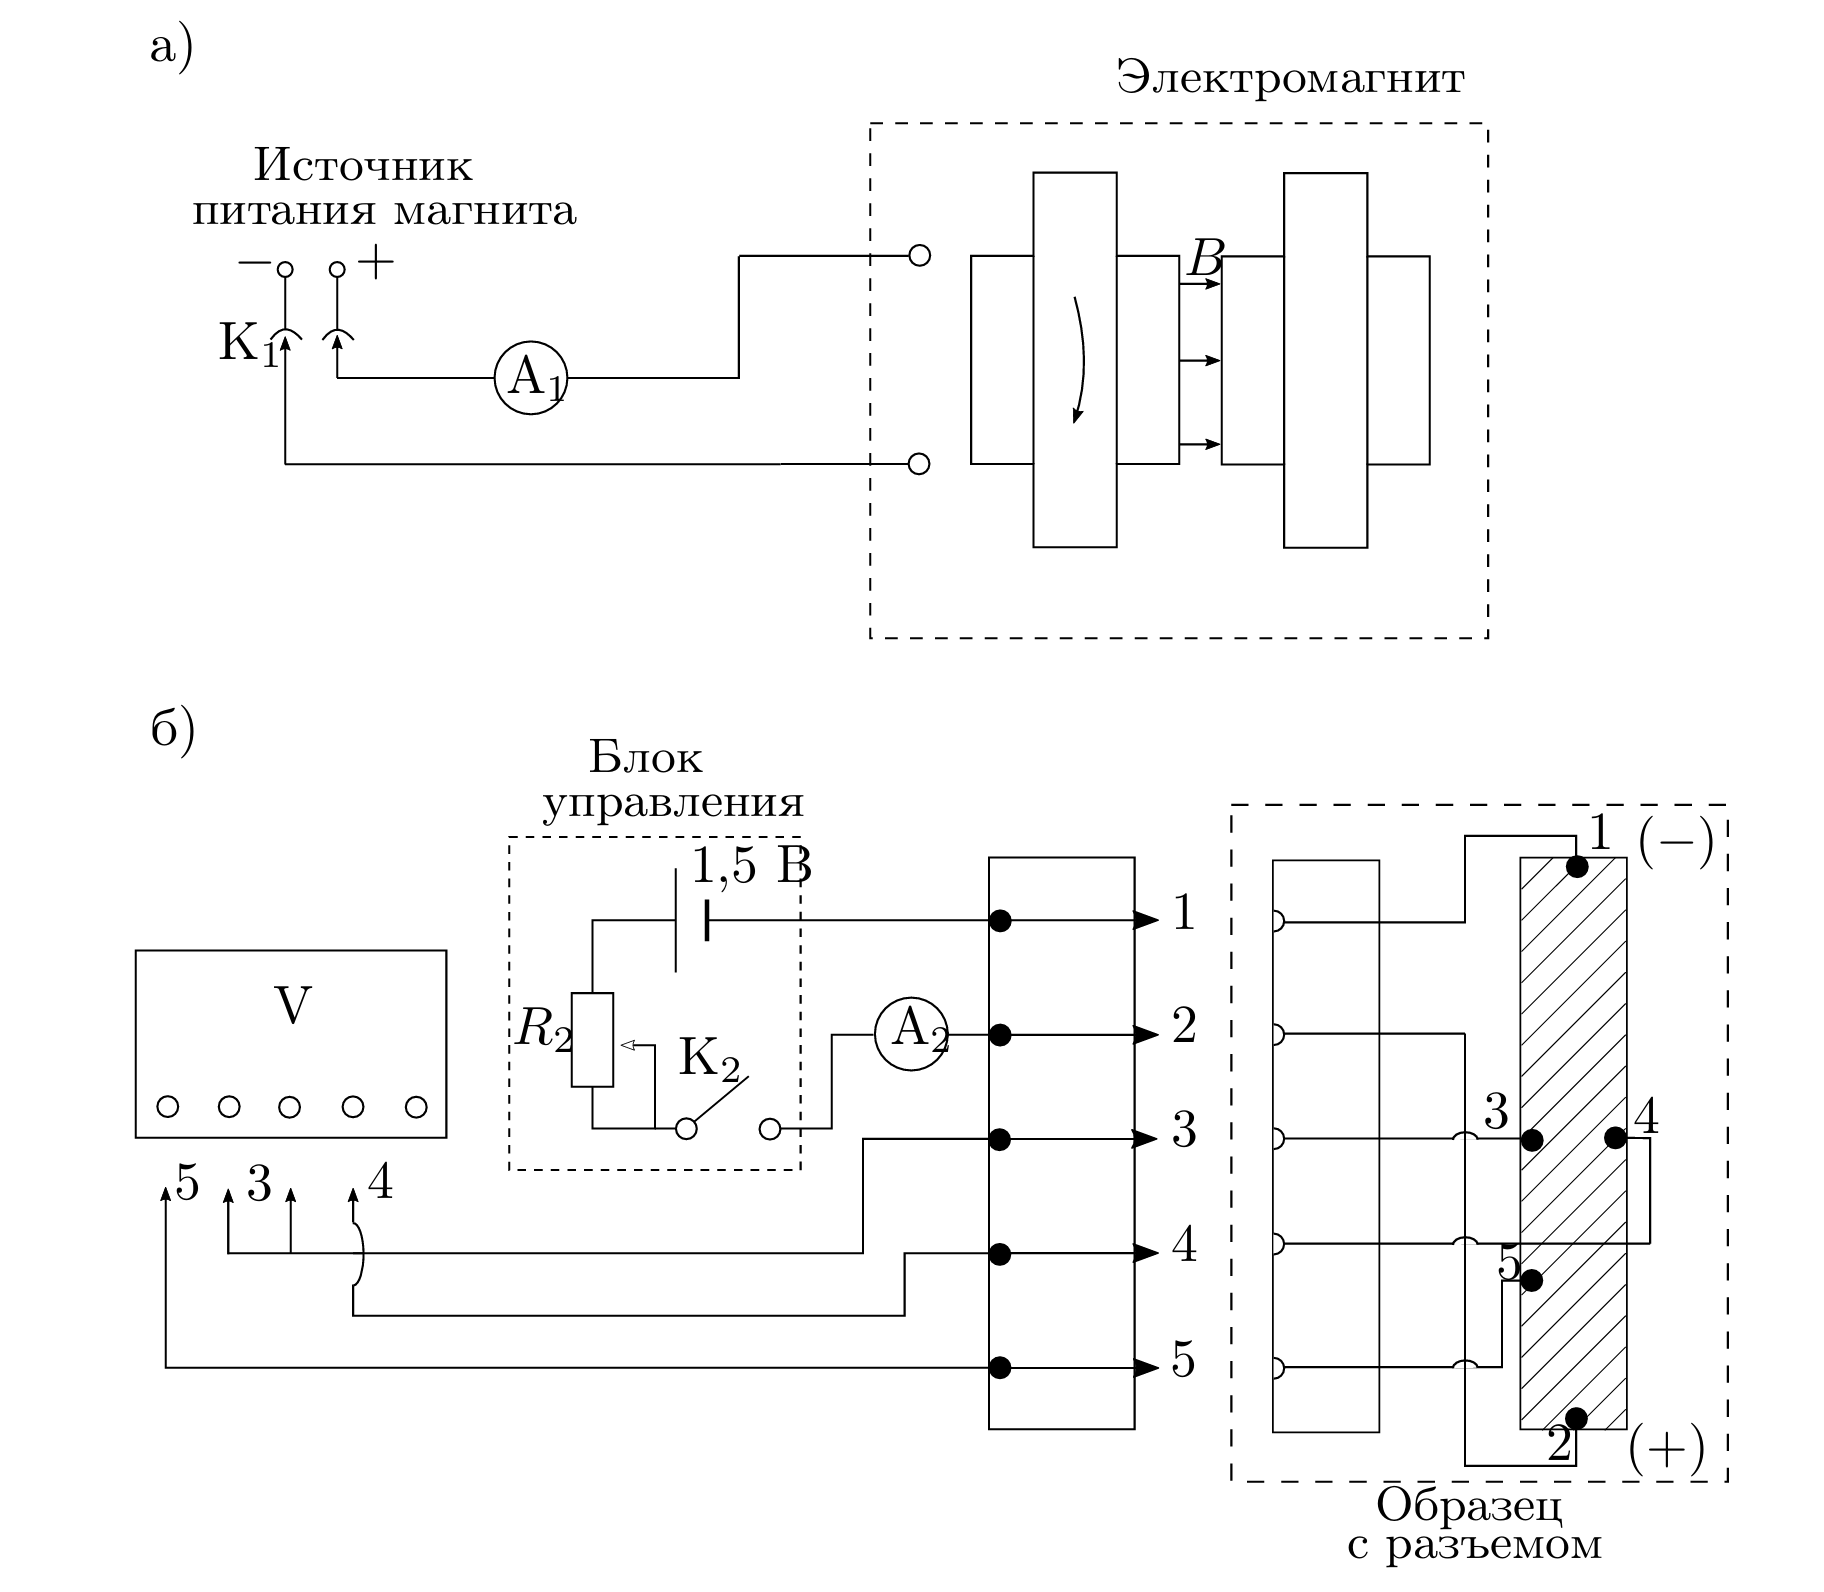
\includegraphics[width=1\linewidth]{setup}
    \caption{Схема установки для исследования эффекта Холла: а) питание электромагнита; б) блок управления и схема подключения образца.}
    \label{fig:setup}
\end{figure*}

Схема установки показана на рис.~\ref{fig:setup}.
Постоянное магнитное поле создаётся в зазоре электромагнита (рис.~\ref{fig:setup}а), ток в обмотках которого $I_M$ плавно меняется регулятором источника питания и измеряется амперметром $A_1$.
Полярность включения магнита меняется разъёмом $K_1$.
Чтобы переводить ток $I_M$ в индукцию поля $B$, проводится предварительная градуировка магнита с помощью миллитесламетра на датчике Холла.

Образец легированного германия в виде прямоугольной пластинки с известными размерами ($a$, $h$, $l$) закреплён в держателе с пятиконтактным разъёмом (рис.~\ref{fig:setup}б).
Токовая цепь питается от источника на $1.5~\text{В}$: при замыкании ключа $K_2$ через торцевые контакты 1 и 2 вдоль образца течёт ток $I$ (не более $1~\text{мА}$), который выставляется реостатом $R_2$ и измеряется миллиамперметром $A_2$.
Разность потенциалов регистрируется цифровым вольтметром $V$.
При измерениях эффекта Холла вольтметр подключается к боковым контактам 3 и 4 (напряжение $U_{34}$), а для нахождения удельного сопротивления образца вне магнита — к контактам 3 и 5 на одной боковой грани (напряжение $U_{35}$).


\section{Ход работы}

\subsection{Параметры образца и градуировка электромагнита}

\begin{figure}[t!]
    \centering
    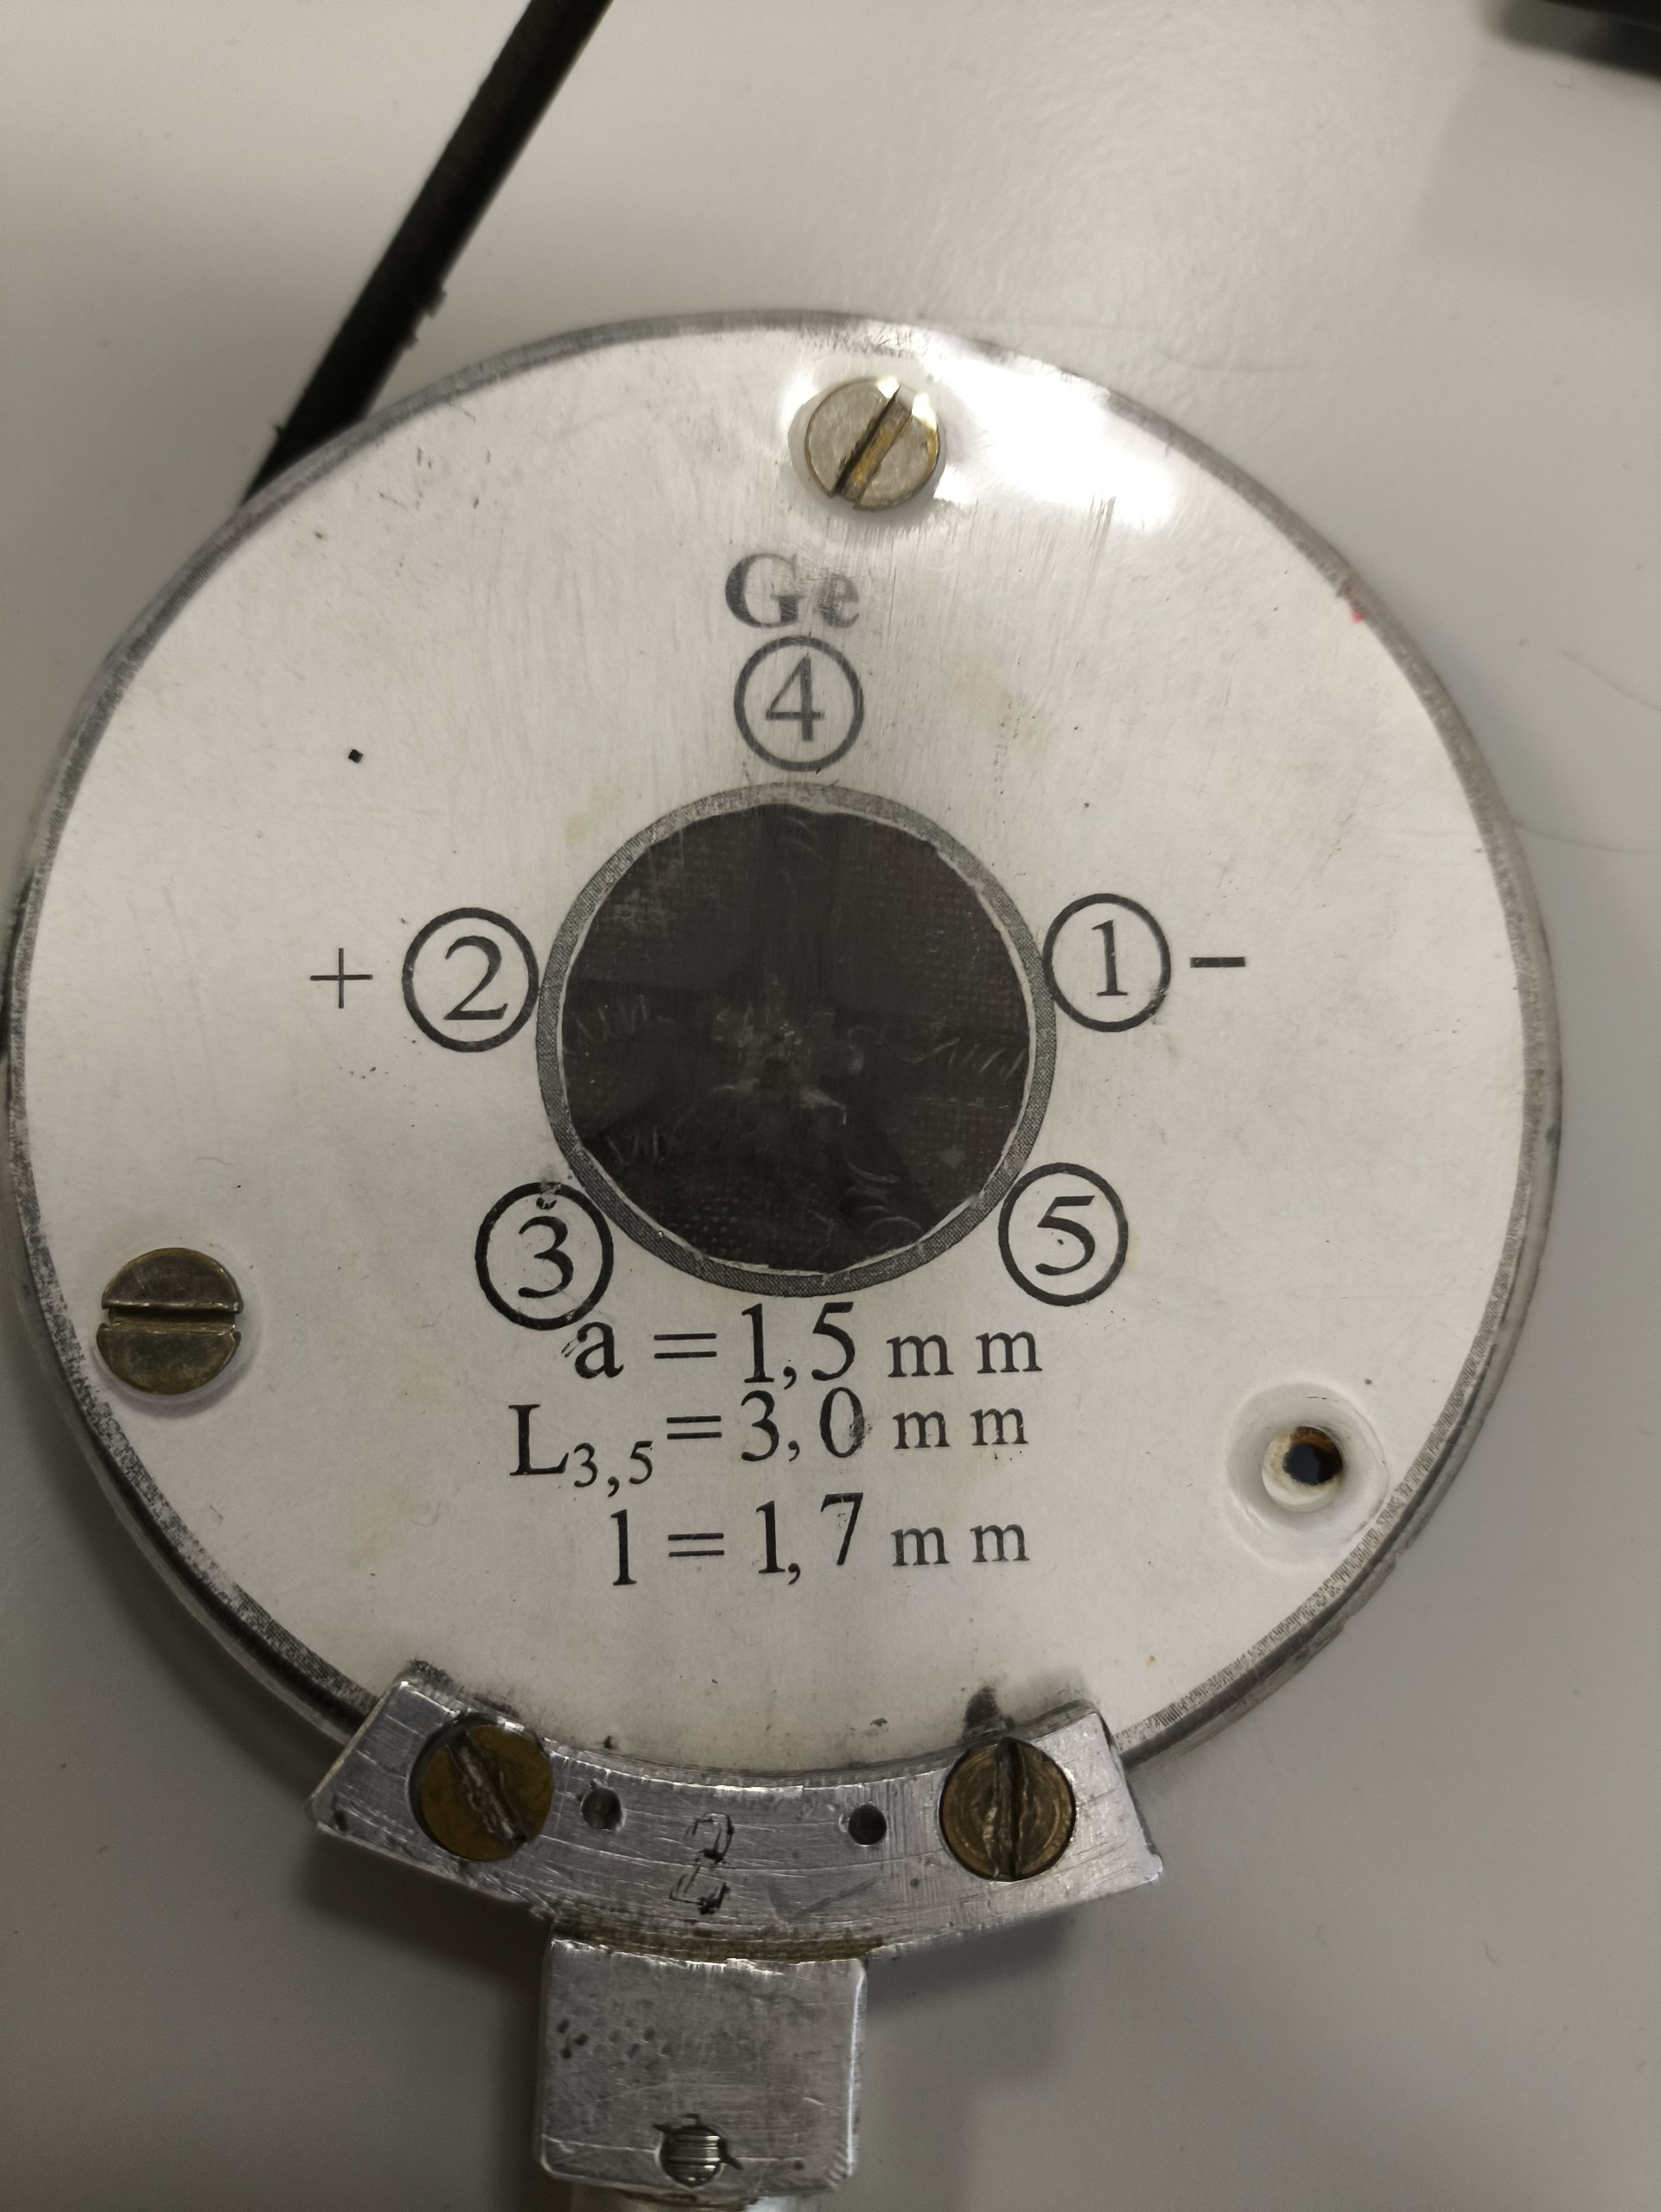
\includegraphics[width=0.65\linewidth]{2.jpg}
    \caption{Внешний вид держателя с образцом легированного германия: расположение токовых ($1$, $2$) и потенциальных ($3$, $4$, $5$) контактов и геометрические параметры пластинки.}
    \label{fig:sample_holder}
\end{figure}

Внешний вид держателя с исследуемым образцом легированного германия показан на рис.~\ref{fig:sample_holder}.
Геометрические размеры пластинки указаны на лицевой панели держателя: ширина образца составляет $a = (1.5 \pm 0.1)~\text{мм}$, расстояние между потенциальными контактами 3 и 5 вдоль пластинки — $l = L_{3,5} = (3.0 \pm 0.1)~\text{мм}$, толщина пластинки (обозначенная на корпусе как $l$) — $h = (1.7 \pm 0.1)~\text{мм}$.
Приборные погрешности оценивались по цене деления и младшему разряду шкал: для цифрового вольтметра при измерении поперечных напряжений $U_{34}$ и $U_0$ погрешность составила $\sigma_U = 1~\text{мкВ}$ (откуда погрешность разности $U_\perp = U_{34} - U_0$ равна $\sigma_{U_\perp} = \sqrt{2}\,\sigma_U \approx 1.41~\text{мкВ}$), при измерении продольного напряжения $U_{35}$ — $0.001~\text{мВ}$, для миллиамперметра $A_2$ в цепи питания образца — $1~\text{дел.} = 0.01~\text{мА}$, для измерителя магнитной индукции — $1\%$. 

\begin{figure}[t!]
    \centering
    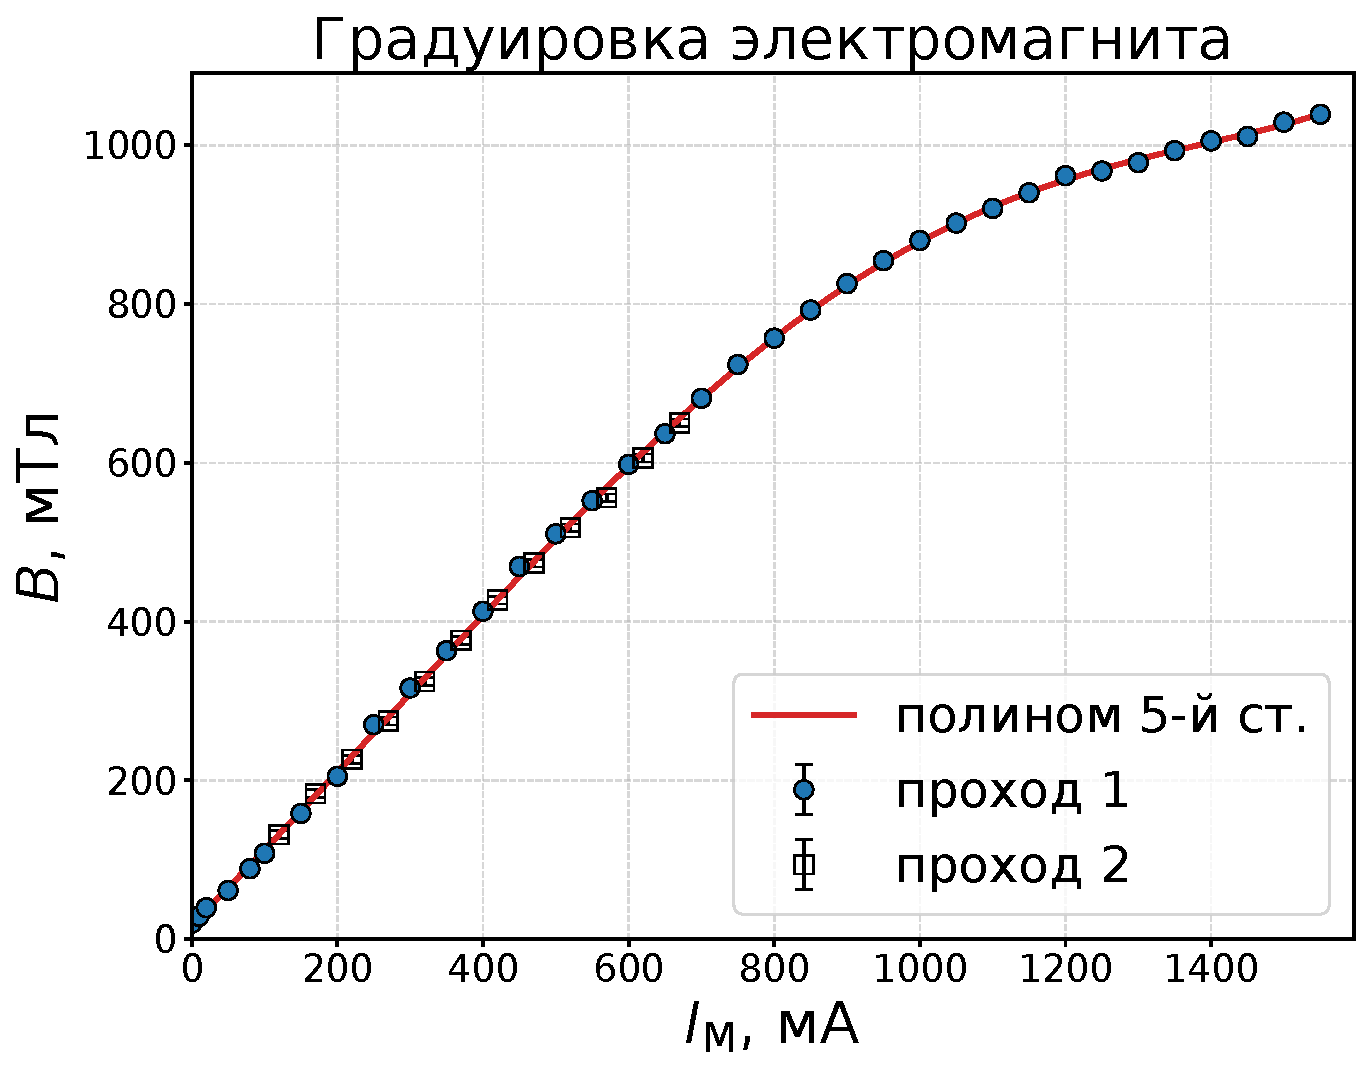
\includegraphics[width=\linewidth]{fig1_calibration_B_of_IM.pdf}
    \caption{Градуировочная кривая электромагнита $B(I_M)$, снятая в два прохода. Сплошная линия — аппроксимация полиномом $5$-й степени, вертикальные усы соответствуют среднеквадратичному разбросу точек $\sigma_B = 4.9~\text{мТл}$.}
    \label{fig:calibration}
\end{figure}

Перед измерениями на образце была проведена градуировка электромагнита во всём рабочем диапазоне токов $I_M$ от $0$ до $1550~\text{мА}$.
В ходе двух проходов было снято $47$ экспериментальных точек, в которых индукция поля $B$ в зазоре менялась от $20$ до $1039~\text{мТл}$ (рис.~\ref{fig:calibration}).
При больших токах $I_M \gtrsim 700~\text{мА}$ зависимость $B(I_M)$ заметно отклоняется от линейной из-за магнитного насыщения стального сердечника.
Для гладкой интерполяции поля калибровочные данные аппроксимировались полиномом $5$-й степени
\begin{equation}
B(I_M) = \sum_{j=0}^{5} c_j I_M^j,
\label{eq:poly_calib}
\end{equation}
степень которого была выбрана как минимальная, после которой среднеквадратичное отклонение (RMS) остатков уменьшается менее чем на $5\%$ (при переходе от $4$-й к $5$-й степени RMS снижается с $5.27$ до $4.93~\text{мТл}$).
Коэффициенты полинома~(\ref{eq:poly_calib}) для $I_M$ в миллиамперах и $B$ в миллитеслах равны: $c_0 = 17.29$, $c_1 = 0.9391$, $c_2 = 1.434 \cdot 10^{-4}$, $c_3 = 6.298 \cdot 10^{-9}$, $c_4 = -3.895 \cdot 10^{-10}$, $c_5 = 1.617 \cdot 10^{-13}$. 

При выключенном токе ($I_M = 0$) в зазоре сохраняется остаточная магнитная индукция $B_{\text{ост}} \approx 17.3~\text{мТл}$ по аппроксимации (непосредственное измерение дало $20~\text{мТл}$). 
Среднее отклонение точек от общей кривой в первом проходе ($35$ точек) составило $+1.3~\text{мТл}$, во втором ($12$ точек) — $-3.8~\text{мТл}$, что отражает слабый гистерезис сердечника; общий разброс $\sigma_B = 4.9~\text{мТл}$ был принят за случайную погрешность калибровки в отдельной точке. 

\subsection{Измерение ЭДС Холла при различных токах}

\begin{table*}[t!]
\caption{Результаты измерений поперечного напряжения $U_{34}$ и ЭДС Холла $U_\perp = U_{34} - U_0$ (в скобках) при различных токах через образец $I$ и токах электромагнита $I_M$. В последней колонке приведены данные для обратного направления магнитного поля ($B < 0$) при $I = 1.30~\text{мА}$.}
\label{tab:raw_data}
\begin{ruledtabular}
\begin{tabular}{cccccccccc}
$I_M$, мА & $B$, мТл & \multicolumn{7}{c}{$U_{34}$ ($U_\perp$), мкВ при прямом поле ($B > 0$)} & $B < 0$ \\
\cline{3-9}
 & & $0.14~\text{мА}$ & $0.25~\text{мА}$ & $0.40~\text{мА}$ & $0.60~\text{мА}$ & $0.80~\text{мА}$ & $1.00~\text{мА}$ & $1.30~\text{мА}$ & $1.30~\text{мА}$ \\
\hline
$0$ ($U_0$) & $17.3$ & $-2$ ($0$) & $-5$ ($0$) & $-12$ ($0$) & $-17$ ($0$) & $-22$ ($0$) & $-28$ ($0$) & $-35$ ($0$) & $-58$ ($0$) \\
$50$ & $64.6$ & $2$ ($4$) & $-2$ ($3$) & $-3$ ($9$) & $-4$ ($13$) & $-8$ ($14$) & $-9$ ($19$) & $-12$ ($23$) & $-83$ ($-25$) \\
$100$ & $112.6$ & $4$ ($6$) & $3$ ($8$) & $4$ ($16$) & $8$ ($25$) & $10$ ($32$) & $13$ ($41$) & $13$ ($48$) & $-106$ ($-48$) \\
$200$ & $210.3$ & $10$ ($12$) & $14$ ($19$) & $22$ ($34$) & $33$ ($50$) & $43$ ($65$) & $55$ ($83$) & $69$ ($104$) & $-162$ ($-104$) \\
$300$ & $309.3$ & $16$ ($18$) & $25$ ($30$) & $40$ ($52$) & $58$ ($75$) & $78$ ($100$) & $99$ ($127$) & $129$ ($164$) & $-221$ ($-163$) \\
$400$ & $408.0$ & $22$ ($24$) & $37$ ($42$) & $57$ ($69$) & $84$ ($101$) & $113$ ($135$) & $140$ ($168$) & $183$ ($218$) & $-280$ ($-222$) \\
$600$ & $595.8$ & $33$ ($35$) & $58$ ($63$) & $88$ ($100$) & $135$ ($152$) & $180$ ($202$) & $223$ ($251$) & $290$ ($325$) & $-387$ ($-329$) \\
$800$ & $757.0$ & $43$ ($45$) & $75$ ($80$) & $118$ ($130$) & $178$ ($195$) & $238$ ($260$) & $297$ ($325$) & $383$ ($418$) & $-486$ ($-428$) \\
$1000$ & $878.3$ & $51$ ($53$) & $88$ ($93$) & $140$ ($152$) & $211$ ($228$) & $281$ ($303$) & $352$ ($380$) & $455$ ($490$) & $-561$ ($-503$) \\
\end{tabular}
\end{ruledtabular}
\end{table*} 

Держатель с образцом помещался в зазор выключенного электромагнита.
Измерения проводились для семи значений тока через образец: $I = 0.14, 0.25, 0.40, 0.60, 0.80, 1.00$ и $1.30~\text{мА}$.
Перед началом каждой серии при $I_M = 0$ фиксировалось напряжение неэквипотенциальности контактов $U_0$, после чего снималась зависимость напряжения $U_{34}$ от тока магнита $I_M$ в диапазоне от $50$ до $1000~\text{мА}$ ($B = 64.6\text{--}878.3~\text{мТл}$).
Исходные данные и вычисленные по формуле~(\ref{eq:u_sub}) значения ЭДС Холла $U_\perp = U_{34} - U_0$ представлены в табл.~\ref{tab:raw_data}.

\begin{figure*}[t!]
    \centering
    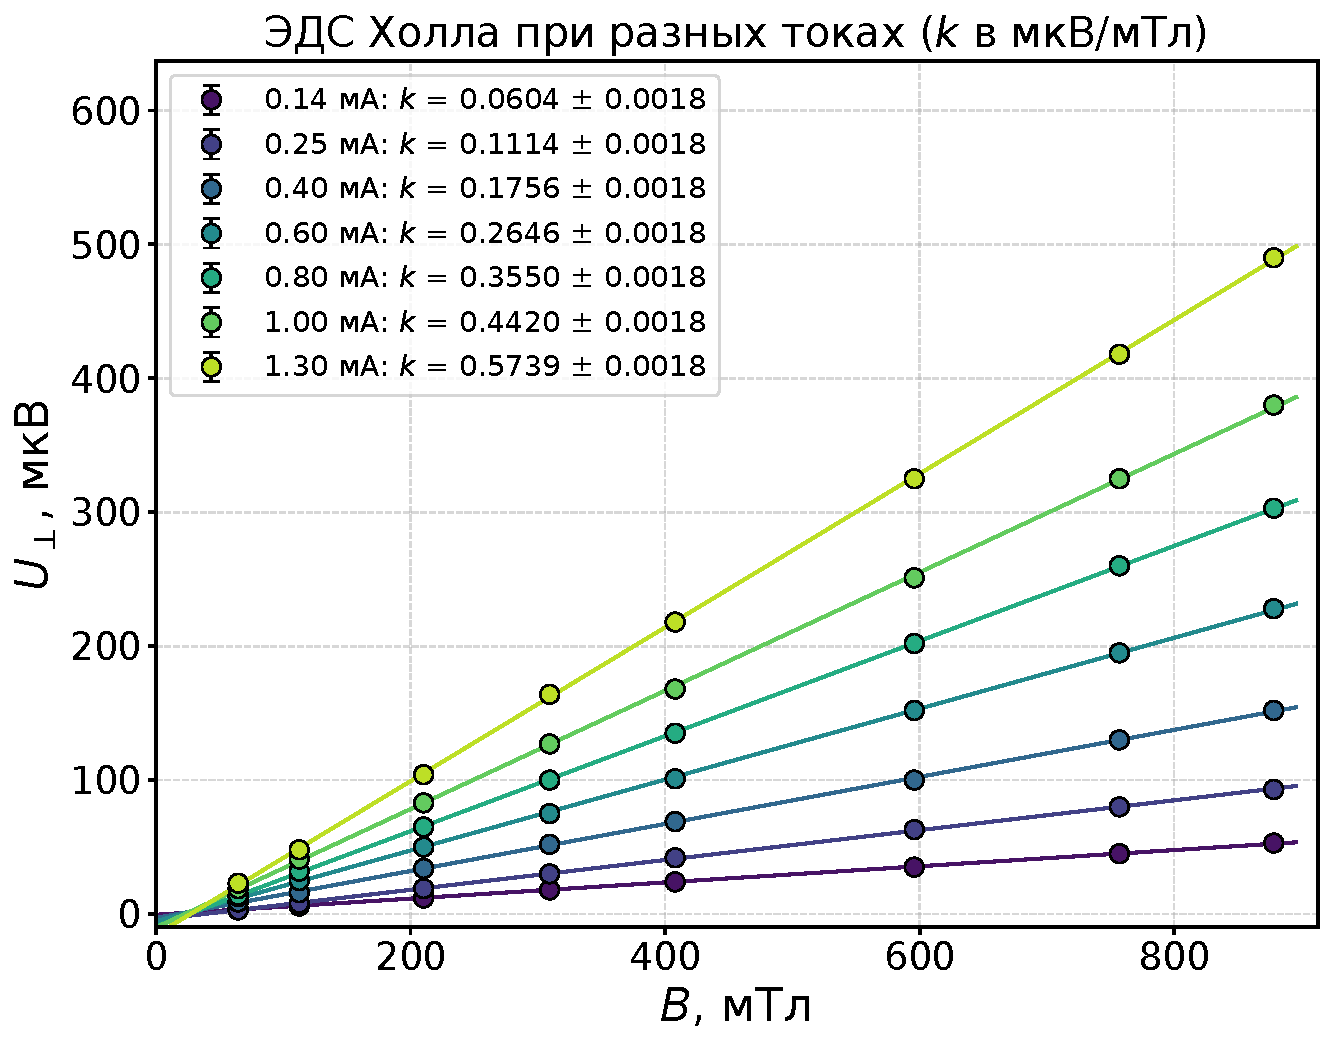
\includegraphics[width=\linewidth]{fig2_hall_family_Uperp_of_B.pdf}
    \caption{Семейство зависимостей ЭДС Холла $U_\perp = U_{34} - U_0$ от магнитной индукции $B$ при различных токах через образец $I$. Прямые линии — линейная аппроксимация методом наименьших квадратов.}
    \label{fig:hall_family}
\end{figure*}

Построенное по этим данным семейство характеристик $U_\perp(B)$ показано на рис.~\ref{fig:hall_family}.
При каждом токе $I$ экспериментальные точки хорошо ложатся на прямую $U_\perp = k B + b$.
Параметры линейной аппроксимации методом наименьших квадратов (МНК) сведены в табл.~\ref{tab:slopes}: среднее по всем сериям приведённое значение $\chi^2/\text{dof}$ составляет $0.58$, что подтверждает применимость линейной модели~(\ref{eq:u_hall}) и отсутствие заметного вклада чётного по полю магнитосопротивления.

\begin{table}[b!]
\caption{Параметры линейной аппроксимации $U_\perp = k B + b$ для различных токов через образец $I$.} 
\label{tab:slopes}
\begin{ruledtabular}
\begin{tabular}{ccccc}
$I$, мА & $U_0$, мкВ & $k$, мкВ/мТл & $b$, мкВ & $\chi^2/\text{dof}$ \\
\hline
$0.14$ & $-2$ & $0.0604 \pm 0.0018$ & $-0.6 \pm 0.9$ & $0.08$ \\
$0.25$ & $-5$ & $0.1114 \pm 0.0018$ & $-4.2 \pm 0.9$ & $0.16$ \\
$0.40$ & $-12$ & $0.1756 \pm 0.0018$ & $-3.0 \pm 0.9$ & $0.41$ \\
$0.60$ & $-17$ & $0.2647 \pm 0.0018$ & $-5.5 \pm 0.9$ & $0.64$ \\
$0.80$ & $-22$ & $0.3550 \pm 0.0018$ & $-9.2 \pm 0.9$ & $0.25$ \\
$1.00$ & $-28$ & $0.4420 \pm 0.0018$ & $-10.1 \pm 0.9$ & $1.34$ \\
$1.30$ & $-35$ & $0.5739 \pm 0.0018$ & $-15.6 \pm 0.9$ & $1.18$ \\
\end{tabular}
\end{ruledtabular}
\end{table}

Систематическое отличие свободного члена $b$ от нуля ($b < 0$, причём $|b|$ растёт с увеличением тока $I$) объясняется остаточной намагниченностью сердечника: поскольку начальное напряжение $U_0$ измерялось при $I_M = 0$, когда в зазоре уже присутствовало поле $B_{\text{ост}}$, разность $U_{34} - U_0$ фактически равна $U_\perp(B) = k(B - B_{\text{ост}})$. 
Оценка остаточного поля по отношению $-b/k$ даёт среднее по сериям значение $(23 \pm 9)~\text{мТл}$, что согласуется с величиной $B(0) \approx 17\text{--}20~\text{мТл}$ из градуировки электромагнита. 
На искомый наклон $k = dU_\perp / dB$ постоянное смещение начала отсчёта не влияет. 

\subsection{Обратное направление магнитного поля и определение типа проводимости}

\begin{figure}[t!]
    \centering
    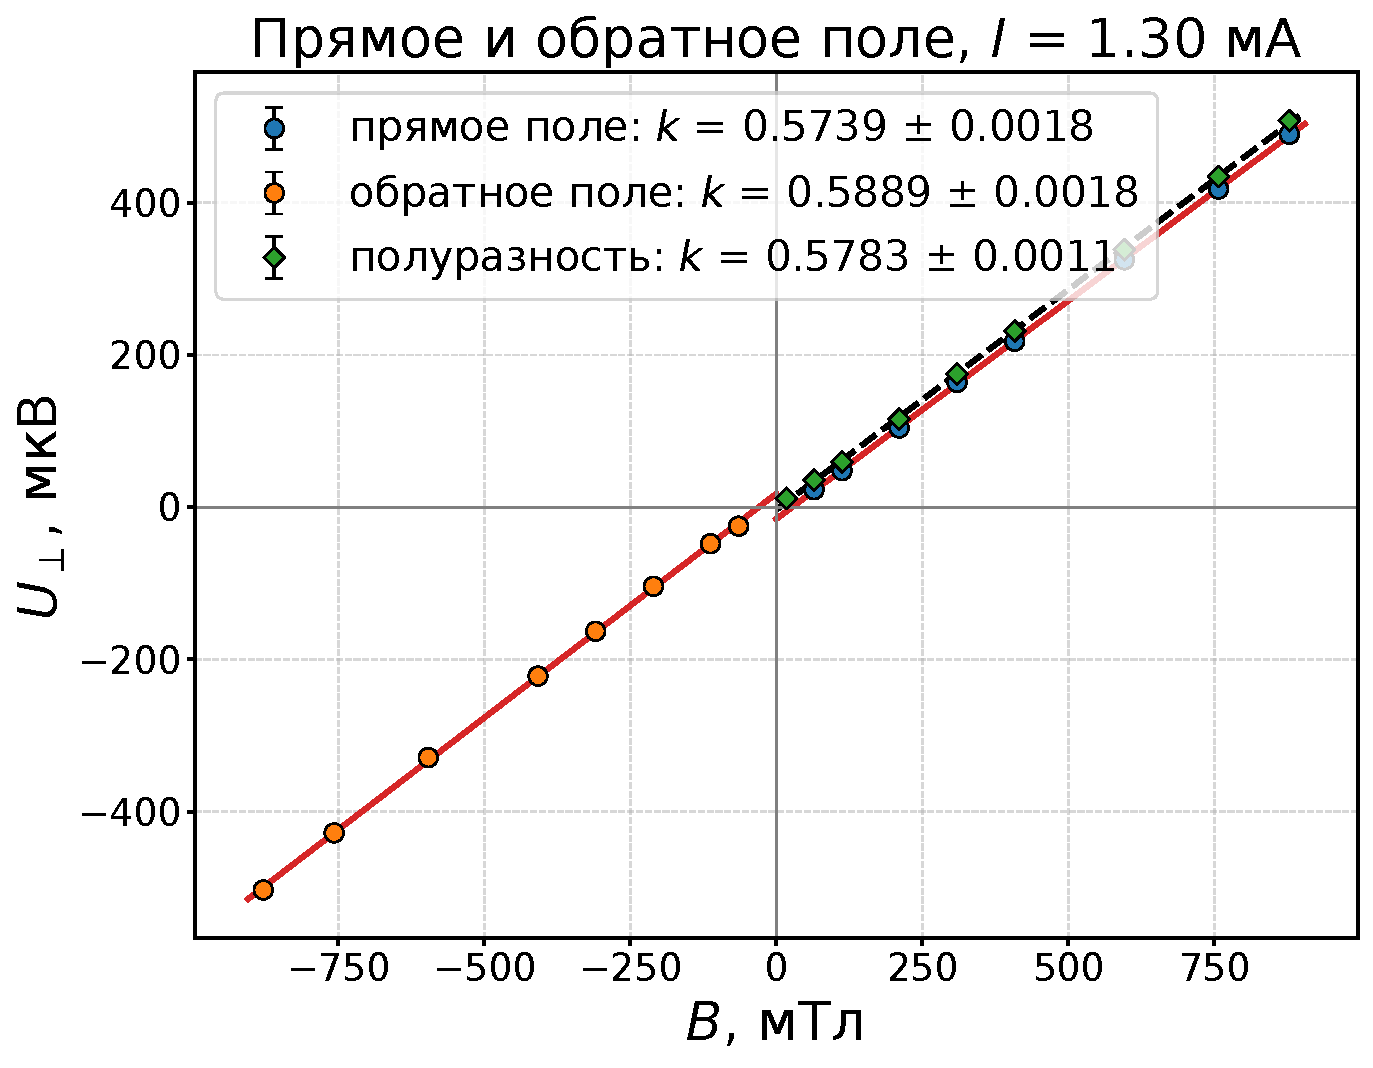
\includegraphics[width=\linewidth]{fig3_reverse_field_check.pdf}
    \caption{Зависимость $U_\perp(B)$ при прямом и обратном направлении магнитного поля для максимального тока $I = 1.30~\text{мА}$. Зелёными ромбами показана ЭДС Холла, найденная методом полуразности~(\ref{eq:u_rev}).}
    \label{fig:reverse}
\end{figure}

При максимальном токе через образец $I = 1.30~\text{мА}$ разъём $K_1$ переключался в обратное положение и снималась зависимость $U_{34}(I_M)$ при противоположном направлении магнитного поля (последний столбец табл.~\ref{tab:raw_data}).
Начальное напряжение при $I_M = 0$ при этом сместилось с $U_0^{(+)} = -35~\text{мкВ}$ до $U_0^{(-)} = -58~\text{мкВ}$, так как остаточное поле сменило знак после перемагничивания сердечника. 

На рис.~\ref{fig:reverse} сопоставлены зависимости $U_\perp(B)$, полученные вычитанием начального напряжения~(\ref{eq:u_sub}) для прямого ($B > 0$) и обратного ($B < 0$) полей, а также значения ЭДС Холла, рассчитанные по формуле полуразности~(\ref{eq:u_rev}) без использования $U_0$.
При инверсии поля поперечное напряжение меняет знак, а точки обоих направлений ложатся практически на одну прямую, проходящую через начало координат, что подтверждает нечётность эффекта по магнитному полю.
Угловой коэффициент составил $k_+ = (0.5739 \pm 0.0018)~\text{мкВ/мТл}$ при прямом поле, $k_- = (0.5889 \pm 0.0018)~\text{мкВ/мТл}$ при обратном поле и $k_{\text{пр}} = (0.5783 \pm 0.0011)~\text{мкВ/мТл}$ по методу полуразности.
Небольшой ненулевой отрезок в методе полуразности ($b = (-3.3 \pm 0.5)~\text{мкВ}$) и расхождение наклонов $k_+$ и $k_-$ на $2.6\%$ обусловлены смещением контактов 3 и 4 при их пайке. Несоосность зондов приводит к проявлению продольного омического падения напряжения и паразитных термоэлектрических эффектов, которые не полностью исключаются при коммутации направления магнитного поля. Половина расхождения наклонов прямого и обратного полей ($1.3\%$) учтена в систематической погрешности постоянной Холла.

\begin{figure}[t!]
    \centering
    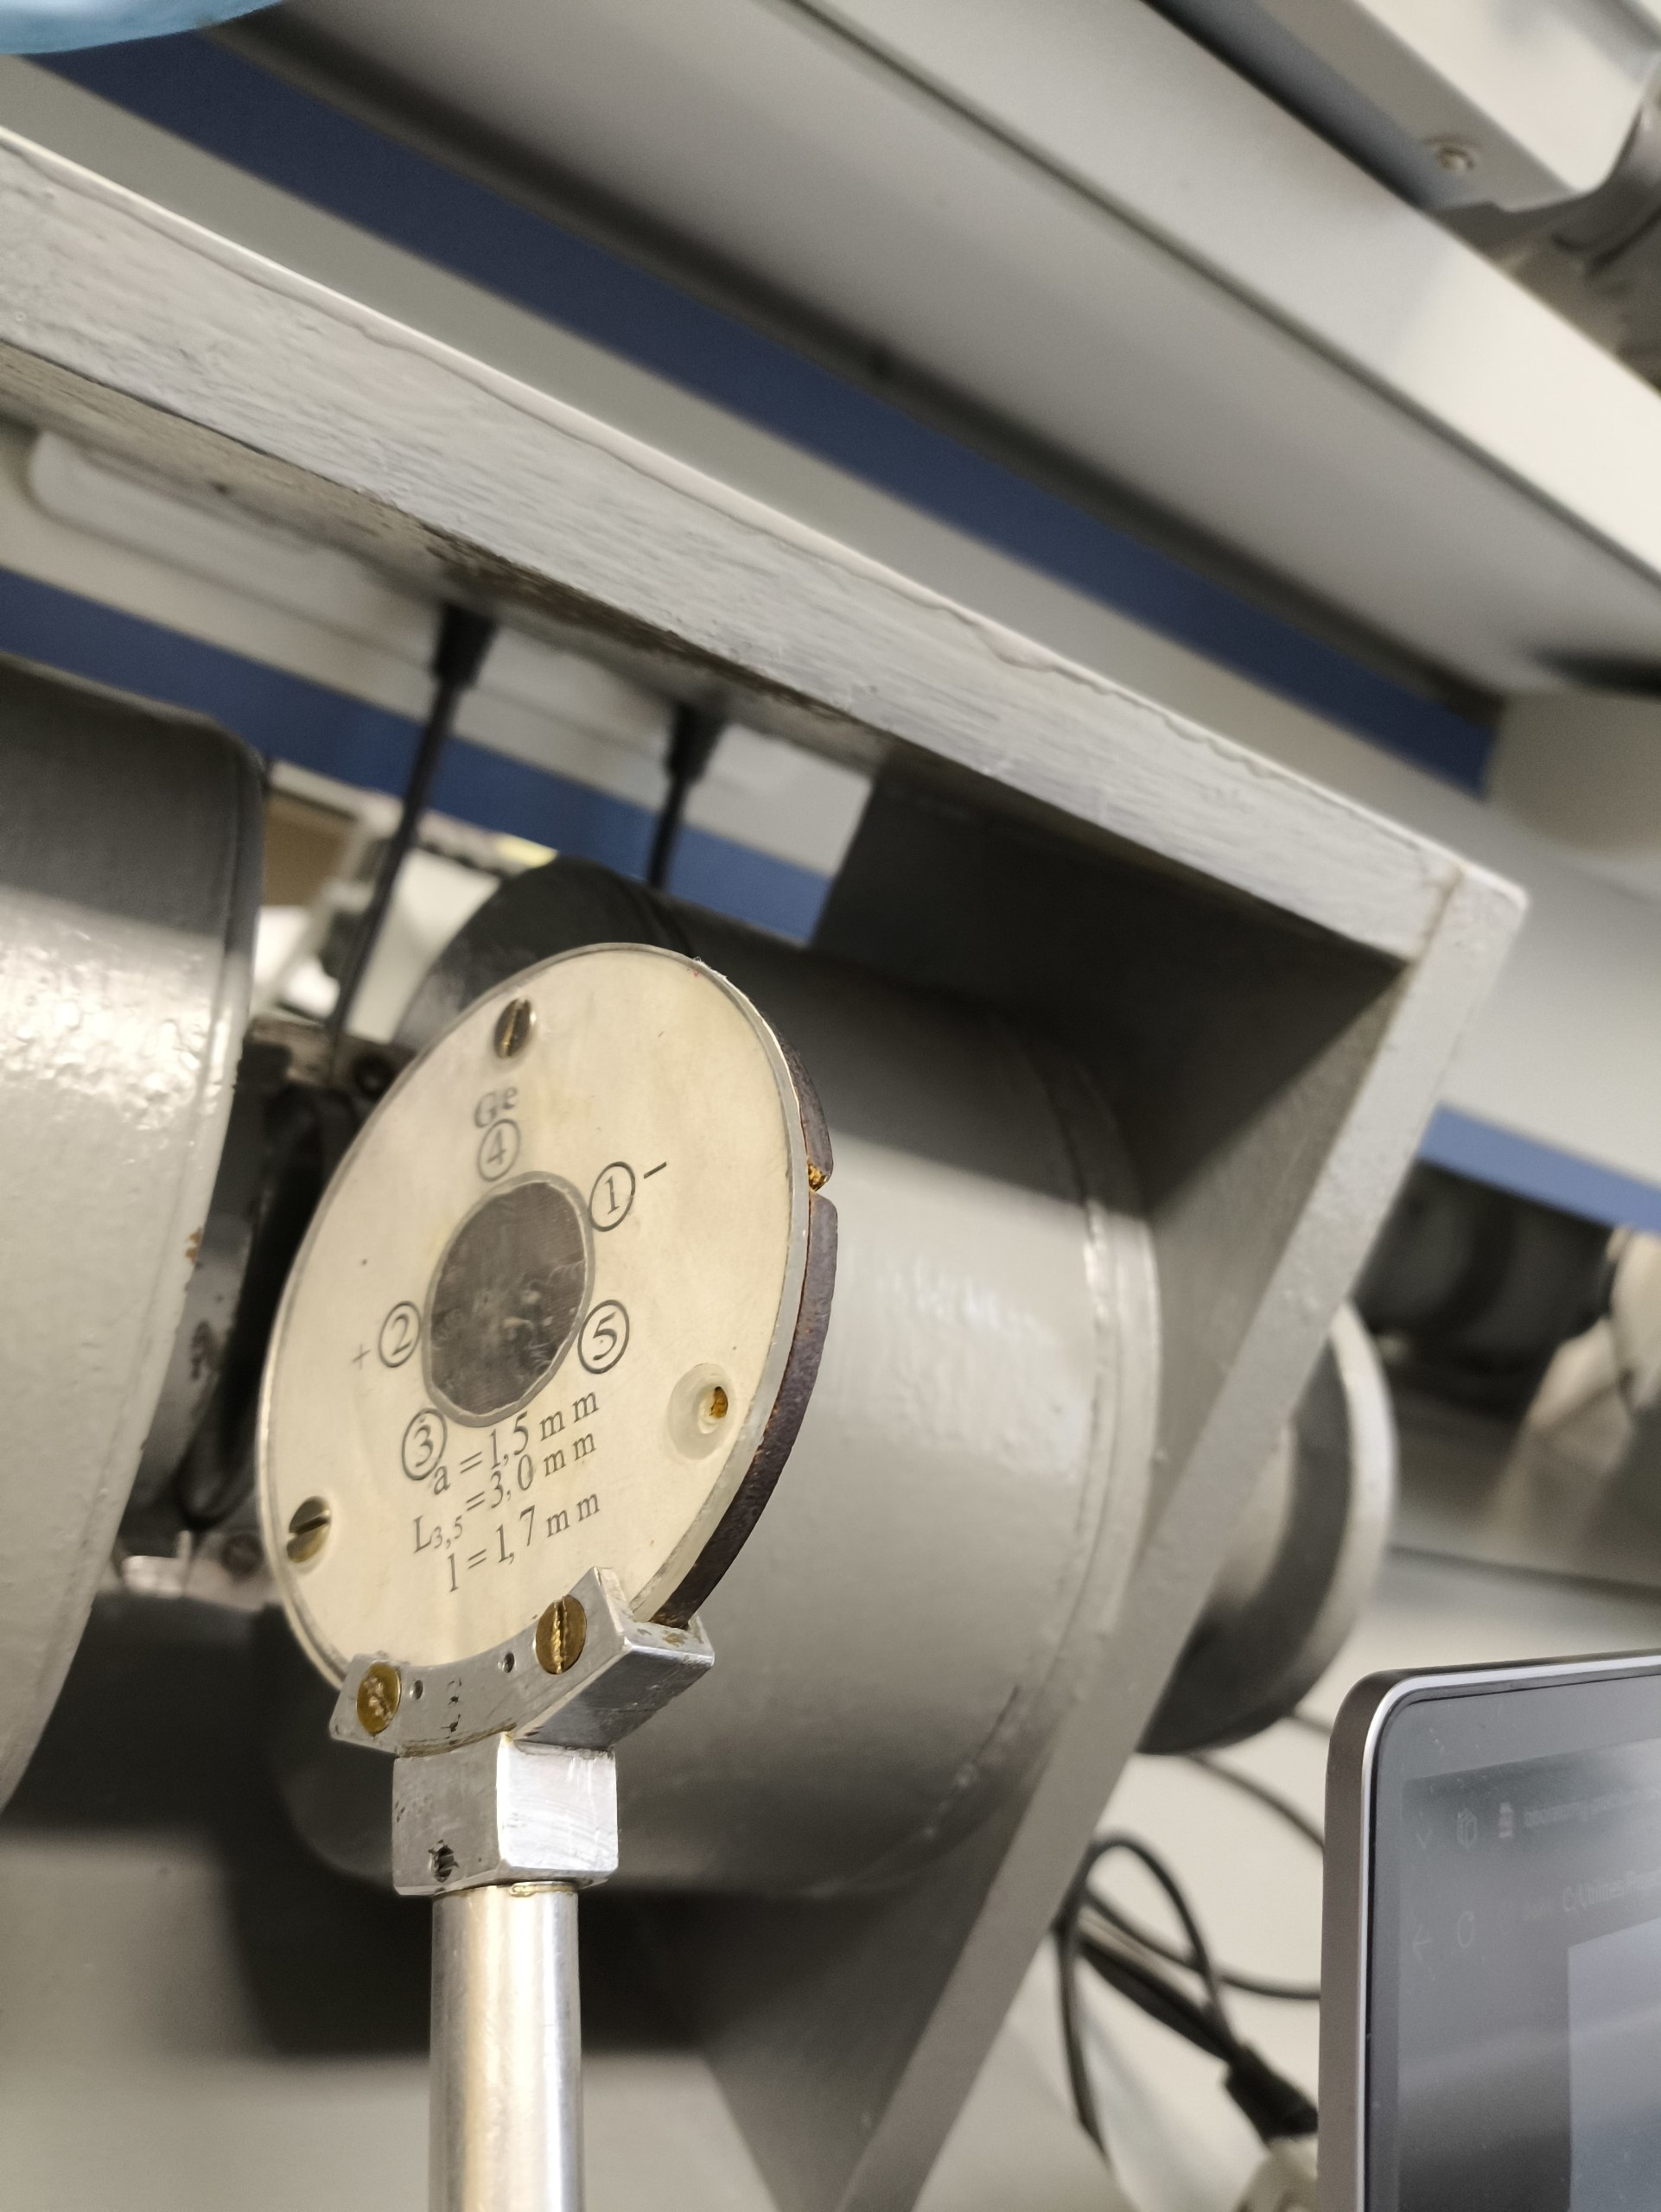
\includegraphics[width=0.48\linewidth]{1.jpg}
    \hfill
    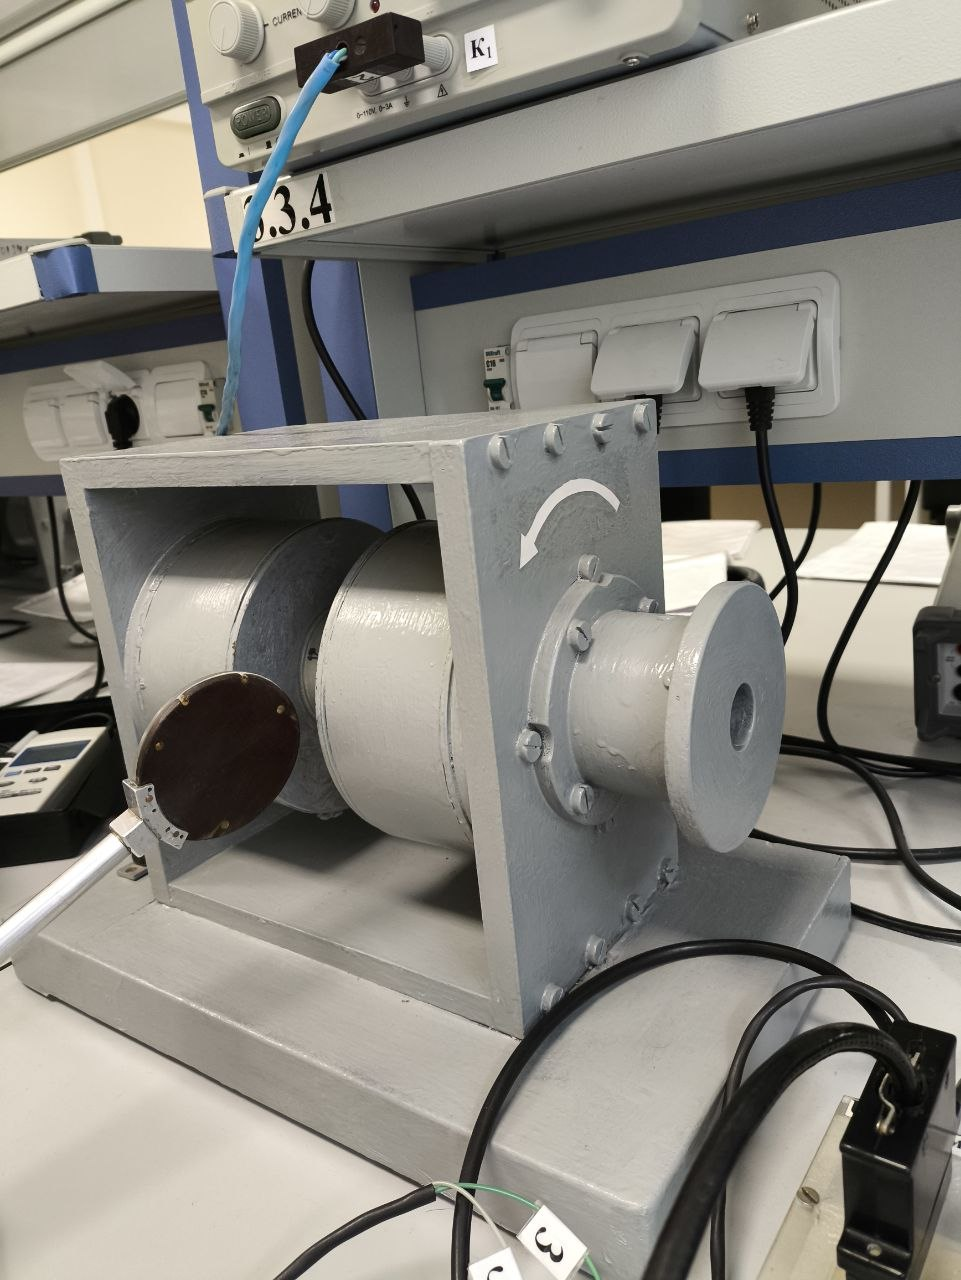
\includegraphics[width=0.48\linewidth]{3.jpg}
    \caption{Расположение держателя с образцом в зазоре электромагнита: вид со стороны лицевой панели с маркировкой контактов (слева) и общий вид относительно катушек со стрелкой направления тока в обмотках (справа).}
    \label{fig:holder_orientation}
\end{figure}

По знаку ЭДС Холла и реальной геометрии установки был определён тип проводимости полупроводника.
Разводка контактов на держателе (рис. 2) отличается от условной схемы на рис.~\ref{fig:setup}б: при взгляде на лицевую сторону держателя рабочий ток $I$ течёт слева направо — от контакта $2$~($+$) к контакту $1$~($-$), при этом холловский контакт $4$ расположен сверху, а контакт $3$ — снизу.
При измерениях держатель устанавливался в зазор электромагнита лицевой панелью к правому полюсу и обратной (текстолитовой) стороной к левому полюсу (рис.~\ref{fig:holder_orientation}).
Направление тока в обмотках при прямом включении разъёма $K_1$ указано белой стрелкой на корпусе магнита (рис.~\ref{fig:holder_orientation}, справа).
При такой ориентации образца в магнитном поле сила Лоренца $\bm{F}_B = q[\bm{v} \times \bm{B}]$ отклоняет носители заряда к нижней боковой грани пластинки (к контакту $3$).
Поскольку в прямом поле во всех сериях измерений разность потенциалов $U_\perp = \varphi_3 - \varphi_4 > 0$ (потенциал контакта $3$ выше потенциала контакта $4$), у нижней грани скапливаются положительно заряженные носители.
Следовательно, исследуемый образец германия обладает дырочной проводимостью ($p$-тип, $R_H > 0$).

\subsection{Определение постоянной Холла, концентрации и подвижности носителей}

\begin{figure}[t!]
    \centering
    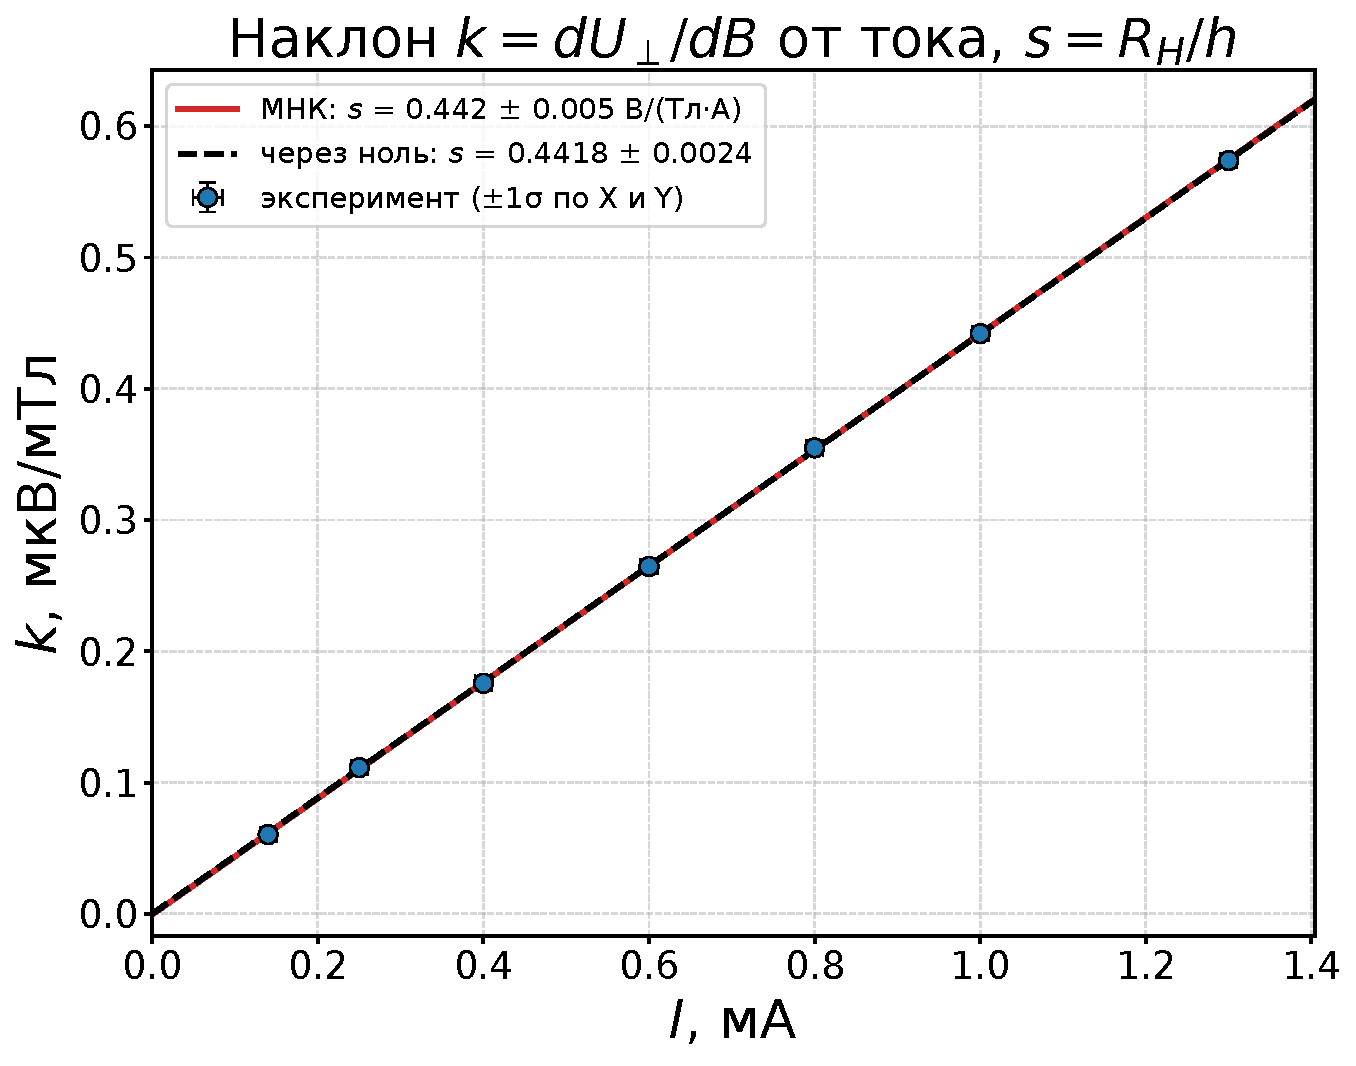
\includegraphics[width=\linewidth]{fig4_k_of_I.pdf}
    \caption{Зависимость углового коэффициента $k = dU_\perp / dB$ от тока через образец $I$. Сплошная красная линия — двухпараметрический МНК, пунктирная — аппроксимация прямой, проходящей через начало координат.}
    \label{fig:k_of_I}
\end{figure}

Для нахождения постоянной Холла по данным табл.~\ref{tab:slopes} был построен график зависимости углового коэффициента $k$ от тока $I$ (рис.~\ref{fig:k_of_I}).
Линейная аппроксимация $k = s I + k_0$ с учётом погрешностей по обеим осям даёт угловой коэффициент
\begin{equation}
s = \frac{dk}{dI} = (0.442 \pm 0.005)~\text{В/(Тл}\cdot\text{А)}
\label{eq:slope_s}
\end{equation}
при свободном члене $k_0 = (-0.0005 \pm 0.0035)~\text{мкВ/мТл}$, который неотличим от нуля в пределах $0.2\sigma$ (однопараметрическая аппроксимация $k = s I$ через начало координат даёт практически то же значение $s = (0.4418 \pm 0.0024)~\text{В/(Тл}\cdot\text{А)}$).
Малая величина $\chi^2/\text{dof} = 0.06$ свидетельствует о том, что точки ложатся на прямую существенно точнее приборной оценки погрешности миллиамперметра ($\sigma_I = 0.01~\text{мА}$). 

Согласно соотношению~(\ref{eq:u_hall}), наклон $s$ равен $|R_H|/h$, откуда с учётом толщины пластинки $h = 1.7~\text{мм}$ и знака носителей постоянная Холла составляет
\begin{equation}
R_H = (750 \pm 50)~\text{см}^3/\text{Кл} = (7.5 \pm 0.5)\cdot 10^{-4}~\text{м}^3/\text{Кл}
\label{eq:rh_res}
\end{equation}
(относительная погрешность $\varepsilon = 6.2\%$). 
Для проверки можно вычислить $|R_H|$ по одной серии измерений при $I = 1.30~\text{мА}$ методом полуразности: $|R_H| = k_{\text{пр}} h / I = (756 \pm 45)~\text{см}^3/\text{Кл}$, что полностью согласуется с результатом~(\ref{eq:rh_res}). 

По формуле~(\ref{eq:r_hall_simple}) для примесного полупроводника с одним типом носителей ($e = 1.60 \cdot 10^{-19}~\text{Кл}$) найдена концентрация электронов проводимости:
\begin{equation}
n = \frac{1}{e |R_H|} = (8.3 \pm 0.5)\cdot 10^{15}~\text{см}^{-3} = (8.3 \pm 0.5)\cdot 10^{21}~\text{м}^{-3}.
\label{eq:n_res}
\end{equation}

Для измерения удельной проводимости держатель с образцом извлекался из зазора электромагнита ($B = 0$).
При максимальном рабочем токе $I = (1.30 \pm 0.01)~\text{мА}$ падение напряжения между контактами 3 и 5 составило $U_{35} = (2.231 \pm 0.001)~\text{мВ}$.
Расчёт по формуле~(\ref{eq:rho}) даёт удельное сопротивление и удельную проводимость легированного германия ($\varepsilon = 9.5\%$):
\begin{align}
\rho_0 &= \frac{U_{35} a h}{I l} = (0.146 \pm 0.014)~\text{Ом}\cdot\text{см}, \label{eq:rho_res} \\
\sigma_0 &= \frac{1}{\rho_0} = (6.9 \pm 0.7)~\text{Ом}^{-1}\cdot\text{см}^{-1}. \label{eq:sigma_res}
\end{align}

Подстановка полученных величин в соотношение~(\ref{eq:mobility}) позволяет определить подвижность электронов в образце:
\begin{equation}
\mu = |R_H|\sigma_0 = \frac{s I l}{U_{35} a} = (5200 \pm 400)~\text{см}^2/(\text{В}\cdot\text{с})
\label{eq:mu_res}
\end{equation}
или $\mu = (0.52 \pm 0.04)~\text{м}^2/(\text{В}\cdot\text{с})$ при относительной погрешности $\varepsilon = 7.7\%$. 
Примечательно, что при выражении подвижности непосредственно через наклон $s$ толщина пластинки $h$ сокращается, поэтому её погрешность ($\varepsilon_h = 5.9\%$) не ухудшает точность определения $\mu$. 

\subsection{Анализ погрешностей, сравнение со справочными данными и микроскопические оценки}
Суммарная относительная погрешность рассчитывалась путём квадратичного сложения независимых приборных и статистических вкладов. 
В погрешность постоянной Холла $R_H$ и концентрации $n$ ($\varepsilon = 6.2\%$) основной вклад вносит неточность знания толщины образца $h$ ($5.9\%$), тогда как статистическая ошибка наклона $s$ составляет всего $1.05\%$, несимметрия переключения поля — $1.29\%$, а погрешность градуировки магнитного поля — около $1.04\%$. 
Аналогично, точность определения $\rho_0$ ($\varepsilon = 9.5\%$) и $\mu$ ($\varepsilon = 7.7\%$) практически целиком лимитируется погрешностями геометрических размеров пластинки $a$ ($6.7\%$), $h$ ($5.9\%$) и $l = L_{3,5}$ ($3.3\%$).

Справочное значение дрейфовой подвижности дырок в чистом германии при комнатной температуре ($T \approx 300~\text{К}$) составляет $\mu_p \approx 1900~\text{см}^2/(\text{В}\cdot\text{с})$ (для электронов $\mu_e \approx 3900~\text{см}^2/(\text{В}\cdot\text{с})$). 
Само по себе легирование полупроводника вводит в решётку заряженные ионы примеси, рассеяние на которых может лишь уменьшить подвижность носителей по сравнению с беспримесным кристаллом.
Тот факт, что полученная в опыте величина $\mu = (5200 \pm 400)~\text{см}^2/(\text{В}\cdot\text{с})$ более чем в $2.5$ раза превышает табличное значение $\mu_p$, объясняется наложением физических и геометрических систематических факторов, присущих методике измерений. 

Во-первых, в справочниках приводится дрейфовая подвижность $\mu_p$, тогда как произведение $|R_H|\sigma_0$ даёт холловскую подвижность $\mu_H = r_H \mu_p$, отличающуюся на кинетический холл-фактор $r_H$.
В германии $p$-типа валентная зона состоит из двух подзон: «тяжёлых» дырок с эффективной массой $m_{hh}^* \approx 0.34\,m_e$ (около $96\%$ всех носителей) и «лёгких» дырок с массой $m_{lh}^* \approx 0.043\,m_e$ (около $4\%$ носителей), подвижность которых примерно в $8$ раз выше. По аналогии с выражением~(\ref{eq:r_hall_two}) для двух сортов носителей одного знака с концентрациями $p_h, p_l$ и подвижностями $\mu_h, \mu_l$ постоянная Холла имеет вид
\begin{equation}
R_H = \frac{r}{e} \frac{p_h \mu_h^2 + p_l \mu_l^2}{(p_h \mu_h + p_l \mu_l)^2}.
\label{eq:r_hall_holes}
\end{equation}
Поскольку подвижности входят в числитель~(\ref{eq:r_hall_holes}) квадратично, даже малая доля быстрых лёгких дырок даёт непропорционально большой вклад в ЭДС Холла. В результате эффективный холл-фактор в $p$-$\text{Ge}$ в слабых и промежуточных магнитных полях возрастает до $r_H \approx 1.8\text{--}2.0$, что физически увеличивает измеряемую холловскую подвижность до $3500\text{--}3800~\text{см}^2/(\text{В}\cdot\text{с})$.

Во-вторых, оставшееся расхождение обусловлено геометрией потенциальных зондов при измерении продольного напряжения $U_{35}$.
Согласно формуле~(\ref{eq:mu_res}), расчётная подвижность пропорциональна отношению $\mu \propto L_{3,5} / (U_{35} a)$.
При малой базе $L_{3,5} = 3.0~\text{мм}$ конечная ширина паяных контактов 3 и 5 ($\sim 0.5~\text{мм}$ каждый) частично шунтирует продольное поле и сокращает реальное расстояние между точками съёма потенциала по сравнению с номинальным.
Кроме того, если торцевые контакты 1 и 2 перекрывают сечение пластинки не полностью, линии тока сгущаются вдоль центральной оси образца, а у боковой грани, где расположены зонды 3 и 5, плотность тока оказывается ниже средней по сечению.
Оба краевых эффекта приводят к систематическому занижению измеряемого падения напряжения $U_{35}$ (и удельного сопротивления $\rho_0$), что завышает вычисляемую проводимость $\sigma_0$ и подвижность $\mu$.
Дополнительный вклад может вносить и отличие фактических размеров кристалла от номинальных значений, нанесённых на корпус держателя.

По найденной подвижности можно также оценить микроскопические параметры транспорта основных носителей (тяжёлых дырок, $m^* \approx 0.34\,m_e \approx 3.1 \cdot 10^{-31}~\text{кг}$) в германии при $T = 295~\text{К}$.
Среднее время свободного пробега составляет $\tau = \mu m^* / e \approx (1.0 \pm 0.1)\cdot 10^{-12}~\text{с}$, что соответствует частоте столкновений $\nu = 1/\tau \approx (1.0 \pm 0.1)\cdot 10^{12}~\text{с}^{-1}$.
При средней тепловой скорости $v_T = \sqrt{3 k_B T / m^*} \approx 2.0 \cdot 10^5~\text{м/с}$ длина свободного пробега равна $\lambda = v_T \tau \approx (200 \pm 15)~\text{нм}$, а коэффициент диффузии по соотношению Эйнштейна составляет $D = \mu k_B T / e = (131 \pm 10)~\text{см}^2/\text{с}$.

% ======================================================================
\section{Заключение}
В работе исследован эффект Холла и продольная электропроводность в образце легированного германия при комнатной температуре.
Проведена градуировка электромагнита в диапазоне полей до $1~\text{Тл}$ и подтверждена линейность зависимости ЭДС Холла от магнитной индукции и тока через образец.
Показано, что как вычитание начального напряжения неэквипотенциальности зондов при нулевом токе магнита, так и метод коммутации направления магнитного поля позволяют эффективно выделить ЭДС Холла на фоне омического падения напряжения.

По знаку холловского напряжения с учётом геометрии контактов держателя установлено, что образец обладает дырочной проводимостью ($p$-тип).
Постоянная Холла составила $R_H = (750 \pm 50)~\text{см}^3/\text{Кл}$, удельное сопротивление $\rho_0 = (0.146 \pm 0.014)~\text{Ом}\cdot\text{см}$, удельная проводимость $\sigma_0 = (6.9 \pm 0.7)~\text{Ом}^{-1}\cdot\text{см}^{-1}$.
Рассчитанные по этим данным концентрация и холловская подвижность основных носителей заряда равны $n = (8.3 \pm 0.5)\cdot 10^{15}~\text{см}^{-3}$ и $\mu = (5200 \pm 400)~\text{см}^2/(\text{В}\cdot\text{с})$.
Превышение измеренной подвижности над справочным значением дрейфовой подвижности для дырочного германия ($\mu_p \approx 1900~\text{см}^2/(\text{В}\cdot\text{с})$) объясняется вкладом подзоны лёгких дырок в постоянную Холла ($r_H > 1$), а также краевыми эффектами и конечным размером потенциальных контактов на малой продольной базе образца.

% --- Библиография ---
\begin{thebibliography}{99}

\bibitem{practicum2019}
Никулин М. Г., Попов П. В., Нозик А. А. и др. \textit{Лабораторный практикум по общей физике. В трёх томах. Т. 2. Электричество и магнетизм} / под ред. А. В. Максимычева, М. Г. Никулина. --- 2-е изд., перераб. и доп. --- М.: МФТИ, 2019.

\end{thebibliography}

\end{document}